\chapter{Concept Bottleneck Model}
\label{concept-bottleneck-pipeline}


% TODO: a introduction to this chapter is useful
% Need to talk about what concept is here

% Things I need to include for Vikranth
%   precision values
%   concepts -> prediction MLP (both old and new)
%   maybe text classification

% What is a concept bottleneck pipeline?
%  - similar results when forcing learning through concepts
%  - interpretability (human-interpretable concepts)

% We build upon this idea by mining concepts from video explanations in lieu of human-generated ones.
% In this section, we show how we have improved upon the concept bottleneck pipeline idea.


Despite their tremendous success in recent years, end-to-end neural networks suffer from their black-box nature.
They enable approximation of unknown functions exceptionally well but provide no interpretation of the actual function being approximated.
The reasoning behind decision-making is almost a necessity in high-risk environments, such as the medical domain, where an error is extremely costly.

Concept Bottleneck Models \cite{RefWorks:RefID:35-koh2020concept} are a recent class of neural networks that tackle the lack of NN interpretability while achieving a competitive performance compared to the end-to-end counterparts. 
The architecture of such a model is shown in \ref{original-concept-bottleneck}.

\begin{figure}[h]
\caption{Schematic representation of the original concept bottleneck pipeline. The input, in this case, is an image but other types of input are also possible.}
\vspace{5pt}
\centering
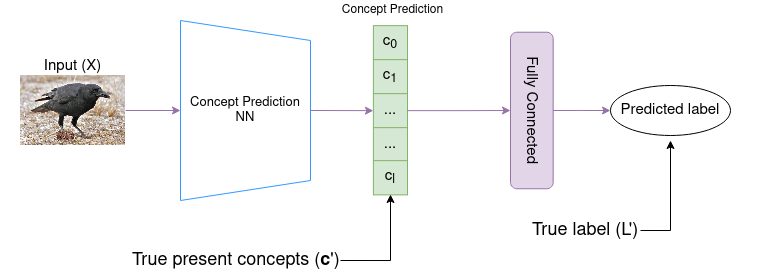
\includegraphics[width=\textwidth]{concept-bottleneck-pipeline/original-concept-bottleneck-model.png}
\label{original-concept-bottleneck}
\end{figure}

An end-to-end NN is transformed into a concept bottleneck one by forcing it to predict human-defined concepts before the final labels.
The final result of the model can then be interpreted by verifying the concepts used when making a decision.
For example, consider a bird prediction problem where human-defined concepts consist of the colour of the beak, wings and body.
If a bird is a crow, the model would predict that it has a black body, wings and beak before indicating that it is a crow.
From those results, an explanation \emph{The bird is a crow because it has black wings, black beak and black body} could be generated.

In this chapter, we take the concept bottleneck idea further.
We mine human-understandable concepts from text explanations of a label in place of a predefined set of concepts.
Such an approach would significantly simplify applying concept bottleneck pipelines in any domain.
It removes the need to predetermine an appropriate set of concepts and manually label all data points where they occur.
Text explanations, on the other hand, are sometimes readily available. For example, we could immediately use a patient's medical history report.
If the explanations are not readily available, they are easy to produce.


% Talk about Vikranth's work
\section{Inherited Work}
\label{inherited-work}

The work on the concept bottleneck pipeline has not been done from scratch.

This chapter itself is a continuation of the ideas proposed by Jeyakumar et al. in \emph{Automatic Concept Extraction for Concept Bottleneck-based Video Classification} \cite{RefWorks:RefID:16-2021automatic}. This paper failed to meet the acceptance threshold for the \href{https://iclr.cc/}{ICLR 2022} conference. 

The main contribution by Jeyakumar et al. is the \emph{Concept Discovery and Extraction Module} (CoDEx), a module that automatically uses explanations to extract text concepts.
That module has been applied to the MLB-V2E dataset, a baseball video dataset with explanations. \\
The architecture involving the \emph{Concept Discovery and Extraction Module} is shown in \ref{vikranth-concept-bottleneck}. 
In general, it is very similar to the standard architecture of the concept bottleneck architecture shown in \ref{original-concept-bottleneck} only with the CoDEx module replacing the true present concepts.

\begin{figure}[h]
\caption{Schematic representation of the concept bottleneck pipeline presented by Jeyakumar et al. (adapted from \cite{RefWorks:RefID:16-2021automatic})} 
\vspace{5pt}
\centering
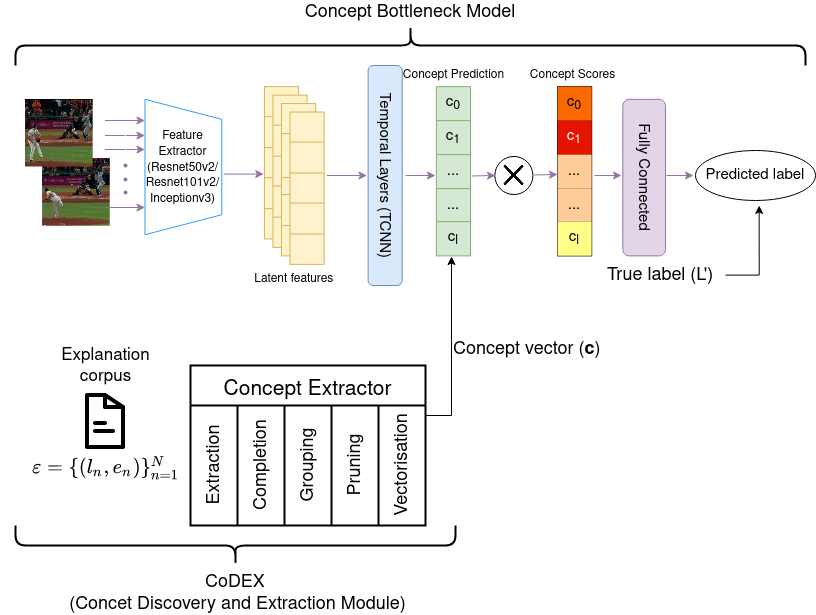
\includegraphics[width=\textwidth]{concept-bottleneck-pipeline/vikranth-concept-bottleneck.png}
\label{vikranth-concept-bottleneck}
\end{figure}


Jeyakumar et al. replace the set of human-crafted present concepts with the output of a CoDEx. 
In addition, to better understand each concept's impact on the final prediction, they add an attention layer after the concept layer to determine the concepts have more impact on the final prediction.
They extract the top three concepts with the highest attention score from that layer, which they use as explanations for a particular label. \\

\emph{Concept Discovery and Extraction Module} design is a vital element of the paper.
The CoDEx presented in the paper consists of 6 stages: \textbf{cleaning}, \textbf{extraction}, \textbf{grouping}, \textbf{completion}, \textbf{pruning}, and \textbf{vectorisation}. \\
The \textbf{cleaning} stage removes videos/explanations which are corrupted. \\
Using a constituency parser and a rule-based methodology, the \textbf{extraction} step determines if a portion of the phrase should be included as a candidate concept. 
The constituency parser uses the rules shown in the following table to extract concepts:

\begin{center}
\begin{tabular}{ |p{2cm}|p{12cm}|  }
 \hline
 \multicolumn{2}{|c|}{Rules determining whether a candidate concept should be included or excluded} \\
 \hline
 rule name & rule \\
 \hline
 Inclusion 1 & noun/pronoun → auxillary (optional) → particle (optional) → verb (optional) \\
 Inclusion 2 & noun/pronoun → auxiliary whose lemma is 'be' → any token \\
 Exclusion & subordinating conjunction \\
 
 \hline
 
\end{tabular}
\label{inclusion-exclusion-rules}
\end{center}

The \textbf{completion} stage looks up for concepts identified in some explanations while not other ones due to the behaviour of the constituency parser.
That stage is done by the substring lookup of existing concepts in all sentences. \\
The \textbf{grouping} step attempts to group concepts with similar meanings using agglomerative clustering \cite{RefWorks:RefID:13-mullner2011modern}.  \\
The \textbf{pruning} stage attempts to keep highly informative concepts by picking the smallest concept subset such that the mutual information \cite{RefWorks:RefID:30-mackay2004information} between the label and a concept vector does not fall below a certain percentage $\gamma$.
This problem is not solved precisely, but rather concepts are inserted using a greedy approach until the mutual information between the label and the newly constructed vector is not below a percentage $\gamma$. The authors chose $\gamma = 0.9$ as an appropriate value. \\
The vectorisation constructs the N x K concept matrix, where K is the number of concepts and N is the number of data points. 
The cell (n, k) is set to one if the concept k occurs for the data point n, zero otherwise.

After all these stages, a binary vector is produced for each data point, which is used in the NN training procedure.
Jeyakumar et al. train the neural network using the joint training approach, where they optimise for both the concept loss and final loss at the same time.
The concept loss is a binary cross entropy loss between a predicted concept vector and CoDEx produced true vector. In contrast, the final loss is a standard categorical cross entropy loss used for classification.

Using the CoDEx and the joint training procedure, the authors showed that their concept bottleneck pipeline had comparable performance to a standard end-to-end model.
In addition, the explanations they extracted were overwhelmingly better than the most common explanations.

% Changes we made to the concept bottleneck pipeline
\section{Adaptions to the Concept Bottleneck Pipeline}

In this chapter, we adapt the CoDEx part of the concept bottleneck pipeline to improve the performance and explainability of the entire model.

The \textbf{extraction} and the \textbf{completion} phase of the CoDEx have been removed from the pipeline.
The former used a rule-based approach to extract concepts.
The latter finds all concepts discovered by the constituency parser in one sentence but not in another using substring matching.

The removed stages are pretty and failed to account for a lot of information the video explanations conveyed.

To replace them extraction and completion we included \textbf{atomisation}, \textbf{generalisation} and \textbf{simple pruning} steps. \\
The chapter \ref{solving-nlp-tasks-logically} explains the first two stages (tasks) in great detail.
The \textbf{atomisation} stage splits provided sentences into one or more atomic sentences. 
Recall that the atomic sentences are sentences which an NLP expert cannot decompose into multiple valid sentences.
This procedure is done using hand-crafted interpretable rules, which are presented in the section \ref{solving-atomisation-task} along with the thought process for choosing the final solution.

The \textbf{generalisation} stage should extract all concept sentences from an atomic one. 
As explained in the section \ref{sentence-type-definitions}, the concept sentence is a syntactically correct sentence obtained by modifying a sentence's syntax tree.
To extract the concept sentences from an atomic sentence, we use a solution learned by ILASP, with the learning procedure described in \ref{solving-generalisation-task}.

The \textbf{simple pruning} stage, included between \textbf{generalisation} and \textbf{grouping} stage, is the simplest out of any of the steps present. 
It removes the concept if it fails to occur at least three times in the dataset.
The sole reason for including this stage is to speed up the subsequent steps because it slightly reduces the overall performance of the pipeline.
% INSERT reference to bird-flowers dataset
CoDEx pipeline for the bird-flowers dataset (\ref{applicability-in-other-domains}) takes less than an hour when the \textbf{simple pruning} stage is not included, which increases to over 10 hours without it.
This stage is only included when the CoDEx pipeline takes too long to compute otherwise because it is lossy.

The diagram summarising the new concept bottleneck pipeline is shown in figure \ref{full-architecture-diagram}.

% TODO: fix X in picture, add boxes for the three parts, missing outlining X as attention module
\begin{figure}[h]
\caption{The entire pipeline for the classification of the MLB-V2E dataset using the concept bottleneck model.} 
\centering
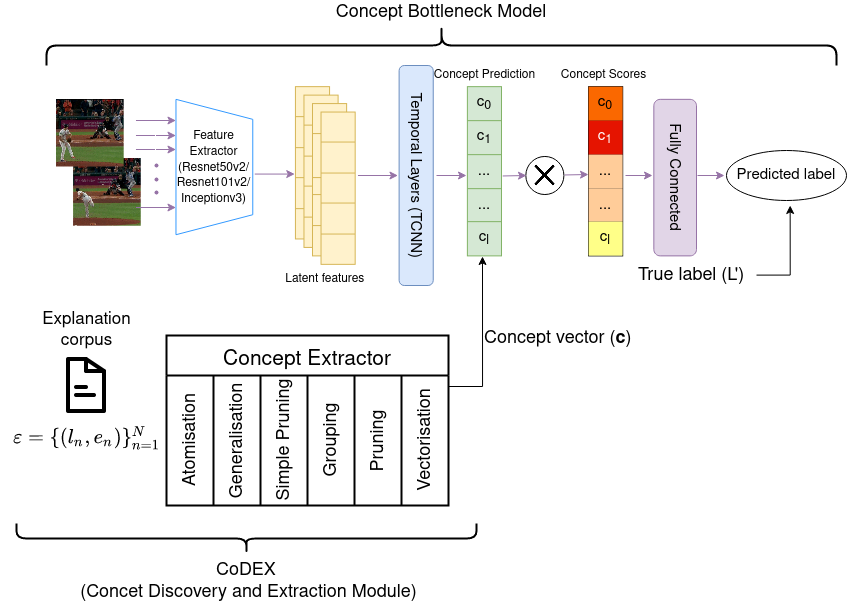
\includegraphics[width=\textwidth]{concept-bottleneck-pipeline/new-concept-bottleneck-pipeline.png}
\label{full-architecture-diagram}
\end{figure}

% INSERT Do cocnept bottlenecks learn as intended
There were recent concerns about the joint training procedure not truly accounting for concepts in their final predictions. 
So, we also attempt to use the sequential training procedure, isolating the training of concept and label prediction parts of the network.
Such a training procedure should perform similarly \cite{RefWorks:RefID:35-koh2020concept}, so we expect the similar results.

\section{Evaluation}

This section will discuss how well the newly presented CoDEx pipeline performs.
Any results produced will be compared with the previous iteration of the concept bottleneck pipeline and the uninterpretable end-to-end model, if applicable.
To keep concept bottleneck pipelines easily comparable, we prune the concepts such that only 78 of them remain.
This number was a desirable value for the original concept bottleneck pipeline \cite{RefWorks:RefID:16-2021automatic}.

Each concept bottleneck model is also trained using both joint and sequential models, unlike the \ref{inherited-work} which only uses the joint model.
% INSERT: Cite "do concept bottleneck models work as intended"
The difference between the two is that the joint optimises losses for both concepts and labels simultaneously, which sometimes overrules the nature of the concept bottleneck pipeline.
The sequential training model freezes the learned concept prediction layers, so the model must determine the final label from the concept predictions themselves.

% INSERT The caltech-ucsd birds-200-2011 dataset, Automated flower classification over a large number of classes
Also, we evaluate the concept bottleneck model on a new birds-flowers dataset, which combines randomly selected images from the CUB-200-2011 and 102 Category Flower Dataset along with their descriptions.
This evaluation inspects how well the concept bottleneck pipeline translates to different domains.

Finally, we will critically analyse the strengths and limitations of the implemented method and suggest areas for future improvement.

\subsection{CoDEx based evaluations}

% INSERT table into the appendix
Tables presenting concept strings for the old and new approaches and their occurrences are shown in Appendix X.

At first glance, both methods extract relevant concepts for the problem, although not all are perfect.
For example, the new method extracts a concept \emph{It was} which is not a relevant concept.
In general, the new method seems to extract concepts which better describe the labels, but we evaluate this belief concretely in this subsection.


\subsubsection{Measuring Cumulative MI}

% INSERT ref MacKay book; maybe insert Venn diagram from Wikipedia.  
Mutual Information $I(X;Y)$ \cite{RefWorks:RefID:30-mackay2004information} is defined as $I(X; Y) \equiv H(X) - H(X|Y)$. 
It estimates the average reduction in uncertainty about $x$ caused by understanding $y$'s value or vice versa. 
It is the average quantity of information conveyed by $x$ regarding $y$.

In the context of this project, the discrete variable $Y$ is a set of label outcomes. A possible outcome is a number between 0 and 4, where each number represents an event which occurred.
The discrete variable $X$ represents a set of extracted concepts with size $k$, where $k$ is a parameter tested in this evaluation.

In addition, given that the cumulative MI is under consideration, the set of size $k$ should ideally contain $k$ \emph{maximally informative} concepts, i.e. those which will result in the highest mutual information score.
However, finding such a set is infeasible as the problem is combinatorial \cite{RefWorks:RefID:16-2021automatic}. Still, we can get a highly informative set by greedily adding a single concept that improves MI the most. 

So, by measuring cumulative MI, we can determine how good the extracted concepts are at describing the labels.

The results can be seen in figure \ref{cummulative-mi-graphs}.

% TODO: replace this with a new version

\begin{figure}[h]
\caption{Cumulative MI graphs using old and new concept extraction pipeline}
\centering
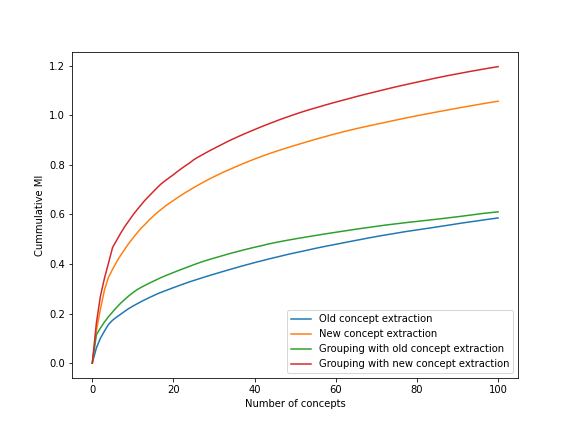
\includegraphics[width=\textwidth]{concept-bottleneck-pipeline/Cummulative MI graphs.png}
\label{cummulative-mi-graphs}
\end{figure}

% TODO: talk about specific numbers

It shows that the new concept extraction method drastically outperforms the old approach for the first 100 concepts.
Since only 78 are taken for the entire pipeline training, these results indicate that the new concept bottleneck performance should drastically improve.


\subsubsection{Concept Prediction Performance}

A corollary of the higher concept mutual information is a higher concept prediction accuracy.

Consider a classifier which would result in the highest possible accuracy for a dataset from binary vectors to labels.
Such a classifier assigns the correct label to any non-conflicting binary vector and the most common label to any conflicting binary vector. 
A conflicting vector is one whose outcome can result in multiple different labels.
The maximum possible accuracies are summarised in the table below:

\begin{center}
\begin{tabular}{ |M{3 cm}||M{3cm}|M{3cm}|  }
 \hline
 \multicolumn{3}{|c|}{Maximum accuracy comparison} \\
 \hline
 \hline
  & Old Concept Extraction&New Concept extraction\\ 
 \hline
 Training dataset & 51.1\% & 78.6\% \\
 Test dataset & 47.7\% & 87.7\% \\
 \hline
\end{tabular}
\end{center}

The highest possible accuracy with the new concept extraction for training and the test set is much greater than the values achievable with the old procedure.

To validate these results translate into practice, we train an MLP classification model from binary vectors to labels with both old and new concept extraction.
% INSERT reference RoBERTa
In addition, a RoBERTa transformer model is trained directly from an unedited human-generated explanation to estimate how much information is lost through concept extraction.
% INSERT: figure comparing transformer MLP with 
The results are presented in the figure \ref{from-concepts-accuracy-comparison}.

\begin{figure}[h]
\caption{Comparison of the label prediction performance from text with a transformer and predicted concepts using MLPs.}
\centering
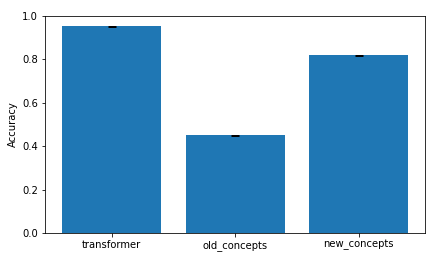
\includegraphics[width=0.5\textwidth]{concept-bottleneck-pipeline/from_explanations_accuracy_comparison.png}
\label{from-concepts-accuracy-comparison}
\end{figure}

These experiments convince us that the performance of a concept bottleneck performance should improve.
They also suggest that there is still room for improvement for the concept extraction since there is a 19\% accuracy improvement by training a model directly from the text.

\subsection{Performance of the Full Concept Bottleneck Pipeline}

The model performance is measured on the entire concept bottleneck pipeline.
We measure the final accuracy of the models with identical architectures using new and old concept extraction. 
In addition, the quality of the concept prediction is also measured as it can help understand whether the concept bottleneck nature of the model is indeed considered. \\
The precision metric is used to measure the concept prediction performance because detecting a subset of present concepts is often enough to determine the final label correctly.
Furthermore, most concept values are set to 0 for any data point, so metrics considering true negatives would have a high value even when the actual concept prediction is poor.
The final label prediction is measured using accuracy, as we want the predictions to be correct most of the time.
The predictive accuracies are also compared with an end-to-end model with an identical architecture, the highest value the concept bottleneck models could achieve.

The model accuracies are presented in the figure \ref{full-process-accuracy-comparison}.
\begin{figure}[h]
\caption{Comparison of the label prediction accuracy for NNs with no, old and new concept prediction in its intermediate layer. The graph on the right is the zoomed-in version of the one on the left to allow observing the differences in performance.}
\centering
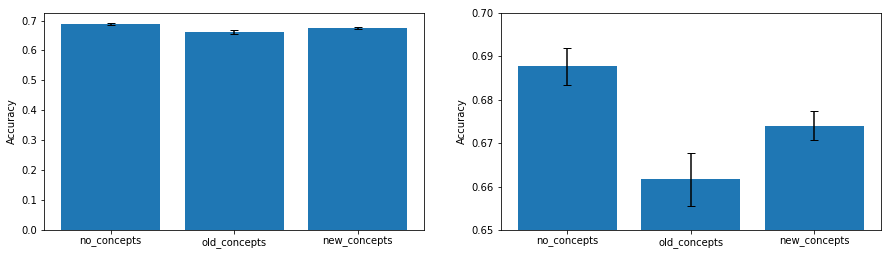
\includegraphics[width=\textwidth]{concept-bottleneck-pipeline/accuracy_comparison.png}
\label{full-process-accuracy-comparison}
\end{figure}

% TODO: analysis of the results
As expected, the model without concepts outperforms both concept bottleneck models. 
In addition, we expect that the new concept extraction outperforms the old one due to the higher mutual information value its concepts have. \\
However, we expected a much more significant performance difference between the concept bottleneck approaches due to a stark contrast in mutual information values.
To understand why that is the case, we need to consider the precision values of the concepts shown in \ref{full-process-concept-precision}.

\begin{figure}[h]
\caption{Comparison of the concept prediction precision score by a NN using old and new concepts in the intermediate layer.}
\centering
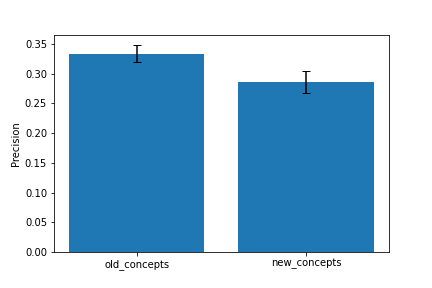
\includegraphics[width=0.5\textwidth]{concept-bottleneck-pipeline/concept_precisions.png}
\label{full-process-concept-precision}
\end{figure}

% TODO: analysis of the resutls
The concept predictions are extremely poor compared to the final results.
So, it is clear that concepts serve more as proxies for holding NN final prediction information instead of genuinely being learned by the network.
% INSERT Do concept bottleneck learn as intended.
This statement is backed up by the fact that old concept prediction even outperforms the prediction results directly from concepts, which would not have been possible in an actual concept bottleneck model (X).

To force the concept bottleneck nature of the model, we use the sequential training approach for the following experiments.
Such an approach first trains the concept prediction part of the network before training the network from concept predictions to final labels.

This approach results in the accuracy results shown in \ref{seq-full-model-results}.

\begin{figure}[h]
\caption{Comparison of the concept prediction precision score by a NN using old and new concepts in the intermediate layer.}
\centering
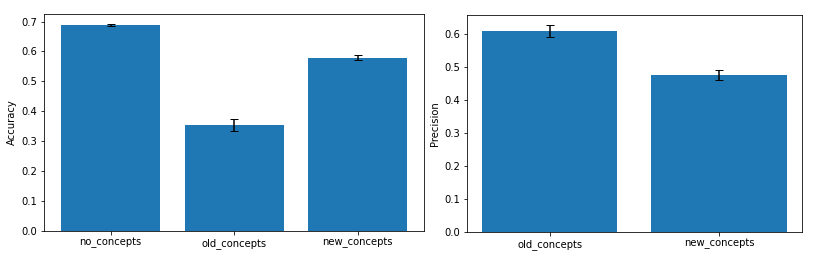
\includegraphics[width=\textwidth]{concept-bottleneck-pipeline/seq_comparison.png}
\label{seq-full-model-results}
\end{figure}

The sequential training has made the results closer to the expectation for the concept bottleneck model. 
There is a more significant difference between models using old and new concepts.
However, despite the concept prediction drastically improving the concept prediction results, they are still poor.
The precision values are still less than 0.5, whose improvement would greatly benefit the final performance too.

\subsection{Explainability of the Labels}


The main reason we use the concept bottleneck pipeline is to allow interpretation of final labels using the intermediate concepts.
To do so, we compare the concept values after attention as human subjects prefer them over all alternatives in almost 70\% of the cases in \cite{RefWorks:RefID:16-2021automatic}.

We consider a concept as active for a data point if it has a score close to the maximum.
This behaviour was chosen because there was a sharp concept value drop of more than 50\% from the few top values, making these concepts lot less relevant for the final decision.


Unfortunately, due to a lack of resources, we have not been able to repeat the Mechanical Turk study done in \cite{RefWorks:RefID:16-2021automatic}. 
Instead, we only discuss three randomly selected test examples and qualitatively compare the old and new concept predictions for them: \\


% Label 1: curr_point = 58, id: WSYKJR5QCQ5K
Sourced explanation 1: \emph{The ball was then fielded and thrown to first base before the batter could make it there. This resulted in an out.}  \\
True label 1: play.

The results are shown in \ref{concepts-results-1}.
The video consisted of a batter hitting a ground ball, which the outfielder threw to the first base, where the base outfielder caught it.
Both networks accurately predict this sequence as a strike.

\begin{figure}[h]
\caption{Most relevant concepts for example 1 along with their concept scores. The LHS shows the ones predicted by the old concept bottleneck, while the RHS is predicted by the new one.}
\centering
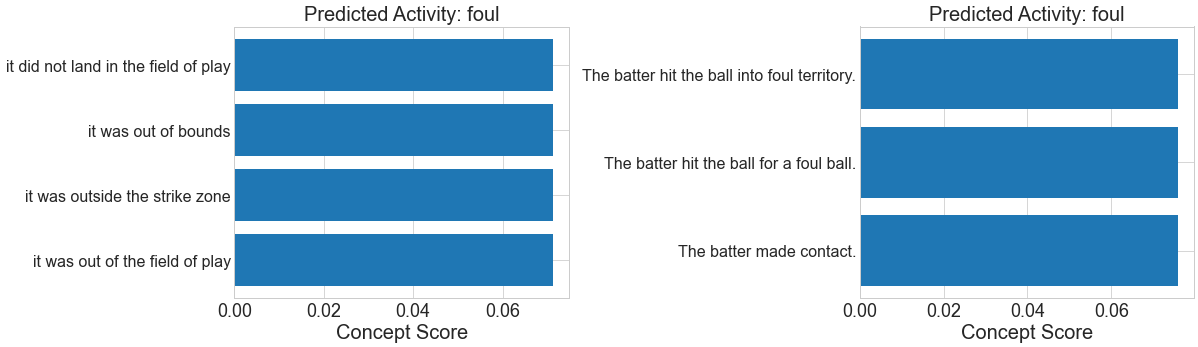
\includegraphics[width=\textwidth]{concept-bottleneck-pipeline/explanations_concepts1.png}
\label{concepts-results-1}
\end{figure}

For the new concept bottleneck network, almost predicted concepts seem correct.
Only the \emph{The batter hit the ball in the air} is not correct.
There also is some redundancy in the outputs. 
For example, sentences \emph{The batter hit a ground ball} and \emph{The batter hit the ball on the ground} mean the same thing.
The grouping stage should merge these cases. \\
On the other hand, the old concept bottleneck model performs worse.
The concept \emph{It was caught} was the only one correctly predicted. 
However, that concept on its own can be very misleading on its own and made to believe that the catcher caught the ball rather than an outfielder.
In a case where the catcher gets the ball, the final label is usually a strike.
The other sentence \emph{The ball went} is unclear about what it describes. \\

% Label 2: curr_point = 73, id: X1J640ZYKXD2
Sourced explanation 2: \emph{Then the outfielder caught it.} \\
True label 2: out

\begin{figure}[h]
\caption{Comparison of the concept prediction precision score by a NN using old and new concepts in the intermediate layer.}
\centering
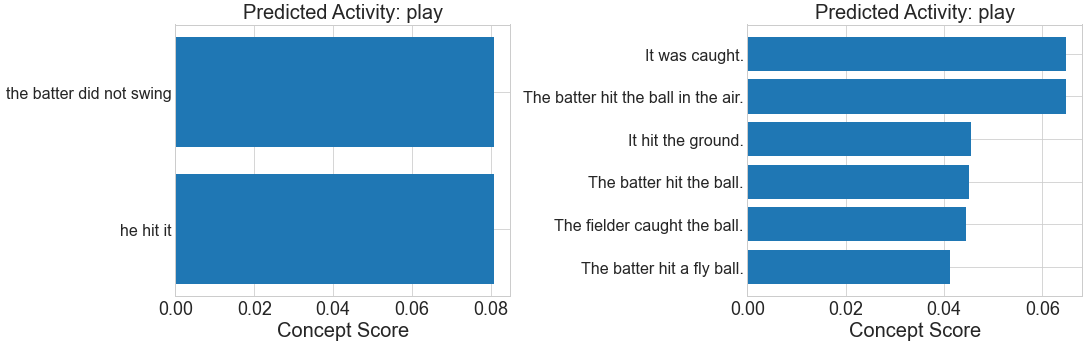
\includegraphics[width=\textwidth]{concept-bottleneck-pipeline/expalantions_concepts2.png}
\label{concepts-results-2}
\end{figure}

The results are shown in \ref{concepts-results-2}.
The video in explanation 2 consisted of the batter hitting the ball in the air, which was caught by an outfielder before hitting the ground.
Both networks accurately predict this sequence as an out.

Unlike the previous video, the final label could be determined by both sets of explanations.
However, the explanation quality and detail are much better for the new concept extraction.
The old method has two good concepts (\emph{It was caught} and \emph{The ball was hit}) while the other two concepts do not describe anything.
The sentence \emph{The pitch was} is also grammatically incorrect.\\
The new concepts capture the fine level of detail exceptionally well. 
One can determine that a fly ball was hit and that the fielder caught the ball.
There is similarly some redundancy as one can determine some concepts through the others \emph{It was caught}.
Its only issue was the explanation \emph{It hit the ground} which did not occur in the video. \\

% Label 3: curr_point = 201, id: ZLP8NFBVSNHS, strike
Sourced explanation 3: \emph{the batter did not swing at a ball in the strike zone}. \\
True label 3: strike

The results are shown in \ref{concept-results-3}.
Only the network with the new concept bottleneck extraction predicted the correct label.

\begin{figure}[h]
\caption{Comparison of the concept prediction precision score by a NN using old and new concepts in the intermediate layer.}
\centering
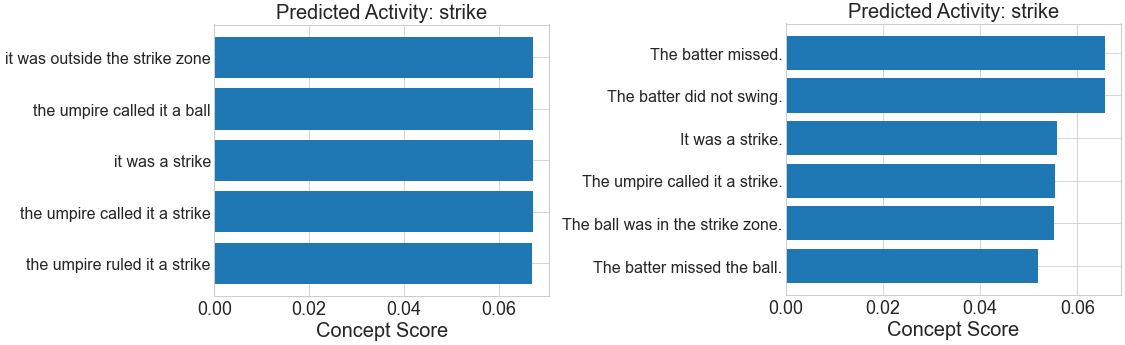
\includegraphics[width=\textwidth]{concept-bottleneck-pipeline/explanations_concepts3.png}
\label{concept-results-3}
\end{figure}

The old concept bottleneck network predicted play as a final label. 
Given that it extracted the same concepts as it did for the first example under consideration, selecting play as a final label is not surprising.
As argued in example 1, the concept \emph{It was caught} without further explanation seems related to the catcher, as was the case here.
The new concept extraction method, on the other hand, extracts all of the concepts correctly. 
It again has some concepts which one could have inferred from another (\emph{The batter missed the ball} and \emph{The batter missed}). \\


To sum up, there seems to be a lot of promise that the new method dramatically improves explanations in terms of accuracy and the level of detail.
We should create a human study in the future to validate these claims.
In addition, notice that most concepts chosen should not actually be predicted since they do not occur in the explanation.
However, they were mostly correct, especially for the new concept extraction.
So, the poor precision value does not necessarily hurt explanations, but rather correct concepts are often not captured by the CoDEx module.

\subsection{Applicability in other Domains}
\label{applicability-in-other-domains}

SKIP this subsection one for now
% TODO: finish

As argued, the idea presented in this section in theory is not tied to video applications.
% INSERT The caltech-ucsd birds-200-2011 dataset, Automated flower classification over a large number of classes, if I can reference descriptions
In this evaluation, we measure how well does the CoDEx module fare when applied to a birds-flowers dataset.
This dataset consists of 2000 birds/flowers images taken from X and X, combined with descriptions generated for these respective datasets.
% INSERT ref results compared to 
It was chosen due to its simplicity for standard NN, as demonstrated by the high accuracy of a non-concept bottleneck model in X.
In addition, the explanations were also readily available to use for concept prediction.

Simply observing the concept we see that the set of concepts extracted may be applicable quite well.
For example, the CoDEx extracts the following concepts together with their occurrence in the dataset:
\begin{verbatim}
The bird has feathers. % 18
This flower has pistil. % 18
\end{verbatim}
Despite the sentence structure immediately highlighting whether it is a bird or a flower, the model would nevertheless try to learn what are feathers and what are pistils.
The issue is the count occurrence for doing so.
Clearly, more than 18 birds in the dataset have feathers, and more than 18 flowers have pistils.
This poor count is a result of label explanations extracted from the two label descriptions focusing on differences between different species of birds/flowers instead of the differences between the two.
In addition, not all concept are useful, such as \emph{This bird has}, but in general there seems to be enough information to determine the final labels correctly.

On the other hand, the concepts produced by the old approach seem much worse. 
It is often quite unclear which label they correspond to, such as \emph{that are oval shaped}.
Or, there is a few very specific concepts which are grouped together of other long concepts.
For example, a concept \emph{this is a white and black bird with a black crown and a long black beak} would fall into that category.

All the extracted concepts are included in Appendix X, 

The count is a result of sentence generalisation, which 



The reason for doing so that these sentences were written to distinguish between bird.
For example, 

The set of concepts extracted may be applicable, for 
The full set of concepts is shown in Appendix X, but we 
The concept extracted by both methods are shown in 

We first compare the accuracy from predicted concepts without any new fine-tuning using both old and new CoDEx modules.
The issue with 

We use RoBERTa transformer trained directly from concept text as a baseline we want to ideally achieve.
% INSERT comparison graph of the results
The results are presented in X.


Clearly 


% TODO: after birds flowers dataset is done

% From concept training

% From concepts transformer training

% Full training


\subsection{Conclusion}

In this chapter, we show that the addition of atomisation and generalisation greatly helps the concept bottleneck pipeline performance.
When incorporated into the concept bottleneck pipeline, the new CoDEx has much higher mutual information,  predictive accuracy, and performance.
In addition, there is an indication that its explanation generation is much better.

We also highlight a possible issue with joint training of a concept bottleneck model that may not truly consider the concept bottleneck nature of the problem.
However, to achieve comparable performance with the sequential training, we need to find a way to capture all the concepts that occur in the video.
